\documentclass{beamer}
\usepackage{tikz}
\usepackage[magyar]{babel}
\usepackage{t1enc}
\usepackage{graphicx}
\usepackage{tikz}
\usepackage{animate}
\usepackage{multimedia}
\usetheme{Goettingen}
\usecolortheme{seahorse}


\title{Időutazás}
\author{Zsigó Bence}
\date{3022. november 23.}

\transduration<13-28>{0}
\begin{document}
\begin{frame}
\maketitle
\end{frame}

\section*{Múltba}
\begin{frame}
\transdissolve
\sectionpage
\end{frame}

\begin{frame}
\transdissolve
\frametitle{Nagypapa-paradoxon}
\centering
\begin{figure}[bt]
\caption{Nagypapa-paradoxon}
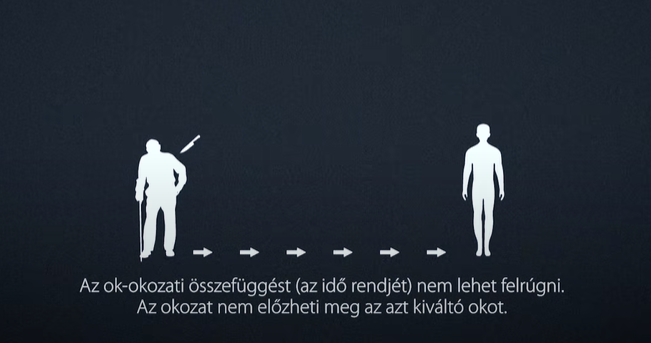
\includegraphics[scale=0.4]{nagypapaparadoxon.png}
\end{figure}
\end{frame}


\begin{frame}
\frametitle{Az érkezési hely meghatározása}
\begin{itemize}
\item Föld tengely körüli forgása, Nap körüli mozgása, a Nap a Galaxisban történő mozgása \pause
\item Szükség lenne a maximális pontosságra \pause
\item Ezért térbeli utazásra is szükség lenne
\end{itemize}
\end{frame}

\begin{frame}
\frametitle{További problémak}
\begin{itemize}
\item Információ a semmiből
\item Anyagáthelyeződés vagy keletkezés
\end{itemize}
\end{frame}

\begin{frame}
\frametitle{Megoldások a paradoxonokra}
\begin{enumerate}
\item Nagypapa-paradoxon
\begin{itemize}
\item Stephen Hawking elméleti fizikus feltételezése szerint egyetlen idővonal létezik, emiatt az időutazó nem képes megváltoztatni a már megtörtént múltat, így nem jöhet létre paradoxon.
\end{itemize} \pause
\item Multiverzum-elmélet
\begin{itemize}
\item Végtelen számú párhuzamosan létező, egymástól különböző, ám összefüggő világegyetem
\item Az időutazás nem más, mint két – eseményeiben független – világegyetem közötti ugrás
\item Az elmélet gyenge pontja a végtelen számú alternatív valóság, amelyekről végtelen ütemben válnak le az újabb alternatív valóságok.
\end{itemize}
\end{enumerate}
\end{frame}

\section*{Jövőbe}
\begin{frame}
\transdissolve
\sectionpage
\end{frame}

\begin{frame}
\transdissolve
\frametitle{Fekete lyuk}
\begin{columns}
\column{0.5\textwidth}
\begin{figure}
\caption{fekete lyuk}
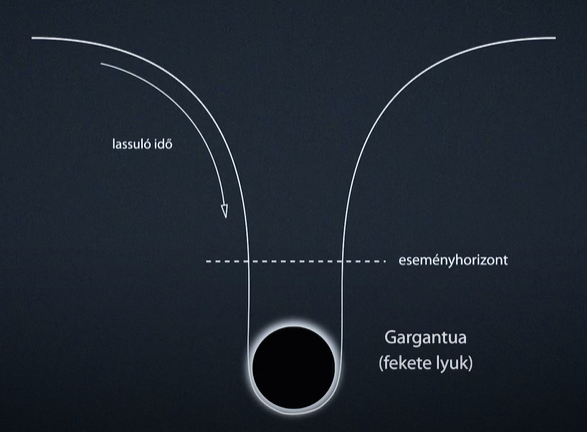
\includegraphics[scale=0.2]{feketelyuk.png}
\end{figure}\pause
\column{0.5\textwidth}
\begin{itemize}
\item A lyuk közepe felé haladva az idő külső szemmel lelassul
\item Az "otthon maradóknak" lassabban telik az idő
\item Pár óra alatt több tíz évet lehetne előre utazni az időben
\end{itemize}
\end{columns}
\end{frame}


\section{fényóra}

\begin{frame}
\frametitle{Fényóra}
\begin{tikzpicture}
\draw (0,5) -- (8,5);
\draw[fill=black] (0,0.2) circle (0.2);
\draw (0,0) -- (8,0);
\end{tikzpicture}
\transduration{0.2}
\end{frame}

\begin{frame}
\frametitle{Fényóra}
\begin{tikzpicture}
\draw (0,5) -- (8,5);
\draw[fill=black] (0,1.1) circle (0.2);
\draw (0,0) -- (8,0);
\end{tikzpicture}
\transduration{0.2}
\end{frame}

\begin{frame}
\frametitle{Fényóra}
\begin{tikzpicture}
\draw (0,5) -- (8,5);
\draw[fill=black] (0,2) circle (0.2);
\draw (0,0) -- (8,0);
\end{tikzpicture}
\transduration{0.2}
\end{frame}

\begin{frame}
\frametitle{Fényóra}
\begin{tikzpicture}
\draw (0,5) -- (8,5);
\draw[fill=black] (0,2.9) circle (0.2);
\draw (0,0) -- (8,0);
\end{tikzpicture}
\transduration{0.2}
\end{frame}

\begin{frame}
\frametitle{Fényóra}
\begin{tikzpicture}
\draw (0,5) -- (8,5);
\draw[fill=black] (0,3.8) circle (0.2);
\draw (0,0) -- (8,0);
\end{tikzpicture}
\transduration{0.2}
\end{frame}

\begin{frame}
\frametitle{Fényóra}
\begin{tikzpicture}
\draw (0,5) -- (8,5);
\draw[fill=black] (0,4.8) circle (0.2);
\draw (0,0) -- (8,0);
\end{tikzpicture}
\transduration{0.2}
\end{frame}

\begin{frame}
\frametitle{Fényóra}
\begin{tikzpicture}
\draw (0,5) -- (8,5);
\draw[fill=black] (0,3.8) circle (0.2);
\draw (0,0) -- (8,0);
\end{tikzpicture}
\transduration{0.2}
\end{frame}

\begin{frame}
\frametitle{Fényóra}
\begin{tikzpicture}
\draw (0,5) -- (8,5);
\draw[fill=black] (0,2.9) circle (0.2);
\draw (0,0) -- (8,0);
\end{tikzpicture}
\transduration{0.2}
\end{frame}

\begin{frame}
\frametitle{Fényóra}
\begin{tikzpicture}
\draw (0,5) -- (8,5);
\draw[fill=black] (0,2) circle (0.2);
\draw (0,0) -- (8,0);
\end{tikzpicture}
\transduration{0.2}
\end{frame}

\begin{frame}
\frametitle{Fényóra}
\begin{tikzpicture}
\draw (0,5) -- (8,5);
\draw[fill=black] (0,1.1) circle (0.2);
\draw (0,0) -- (8,0);
\end{tikzpicture}
\transduration{0.2}
\end{frame}

\begin{frame}
\frametitle{Fényóra}
\begin{tikzpicture}
\draw (0,5) -- (8,5);
\draw[fill=black] (0,0.2) circle (0.2);
\draw (0,0) -- (8,0);
\end{tikzpicture}
\transduration{0.2}
\end{frame}

\begin{frame}
\frametitle{Fényóra}
\begin{tikzpicture}
\draw (0,5) -- (8,5);
\draw[fill=black] (0,1.1) circle (0.2);
\draw (0,0) -- (8,0);
\end{tikzpicture}
\transduration{0.2}
\end{frame}

\begin{frame}
\frametitle{Fényóra}
\begin{tikzpicture}
\draw (0,5) -- (8,5);
\draw[fill=black] (0,2) circle (0.2);
\draw (0,0) -- (8,0);
\end{tikzpicture}
\transduration{0.2}
\end{frame}

\begin{frame}
\frametitle{Fényóra}
\begin{tikzpicture}
\draw (0,5) -- (8,5);
\draw[fill=black] (0,2.9) circle (0.2);
\draw (0,0) -- (8,0);
\end{tikzpicture}
\transduration{0.2}
\end{frame}

\begin{frame}
\frametitle{Fényóra}
\begin{tikzpicture}
\draw (0,5) -- (8,5);
\draw[fill=black] (0,3.8) circle (0.2);
\draw (0,0) -- (8,0);
\end{tikzpicture}
\transduration{0.2}
\end{frame}

\begin{frame}
\frametitle{Fényóra}
\begin{tikzpicture}
\draw (0,5) -- (8,5);
\draw[fill=black] (0,4.8) circle (0.2);
\draw (0,0) -- (8,0);
\end{tikzpicture}
\transduration{0.2}
\end{frame}

\begin{frame}
\frametitle{Fényóra}
\begin{tikzpicture}
\draw (0,5) -- (8,5);
\draw[fill=black] (0.25,3.6) circle (0.2);
\draw (0,0) -- (8,0);
\end{tikzpicture}
\transduration{0.2}
\end{frame}

\begin{frame}
\frametitle{Fényóra}
\begin{tikzpicture}
\draw (0,5) -- (8,5);
\draw[fill=black] (0.5,2.5) circle (0.2);
\draw (0,0) -- (8,0);
\end{tikzpicture}
\transduration{0.2}
\end{frame}

\begin{frame}
\frametitle{Fényóra}
\begin{tikzpicture}
\draw (0,5) -- (8,5);
\draw[fill=black] (0.75,1.4) circle (0.2);
\draw (0,0) -- (8,0);
\end{tikzpicture}
\transduration{0.2}
\end{frame}

\begin{frame}
\frametitle{Fényóra}
\begin{tikzpicture}
\draw (0,5) -- (8,5);
\draw[fill=black] (1,0.2) circle (0.2);
\draw (0,0) -- (8,0);
\end{tikzpicture}
\transduration{0.2}
\end{frame}

\begin{frame}
\frametitle{Fényóra}
\begin{tikzpicture}
\draw (0,5) -- (8,5);
\draw[fill=black] (1.5,0.6) circle (0.2);
\draw (0,0) -- (8,0);
\end{tikzpicture}
\transduration{0.2}
\end{frame}

\begin{frame}
\frametitle{Fényóra}
\begin{tikzpicture}
\draw (0,5) -- (8,5);
\draw[fill=black] (2,1) circle (0.2);
\draw (0,0) -- (8,0);
\end{tikzpicture}
\transduration{0.2}
\end{frame}

\begin{frame}
\frametitle{Fényóra}
\begin{tikzpicture}
\draw (0,5) -- (8,5);
\draw[fill=black] (2.5,1.4) circle (0.2);
\draw (0,0) -- (8,0);
\end{tikzpicture}
\transduration{0.2}
\end{frame}

\begin{frame}
\frametitle{Fényóra}
\begin{tikzpicture}
\draw (0,5) -- (8,5);
\draw[fill=black] (3,1.8) circle (0.2);
\draw (0,0) -- (8,0);
\end{tikzpicture}
\transduration{0.2}
\end{frame}

\begin{frame}
\frametitle{Fényóra}
\begin{tikzpicture}
\draw (0,5) -- (8,5);
\draw[fill=black] (4,1.9) circle (0.2);
\draw (0,0) -- (8,0);
\end{tikzpicture}
\transduration{0.2}
\end{frame}

\begin{frame}
\frametitle{Fényóra}
\begin{tikzpicture}
\draw (0,5) -- (8,5);
\draw[fill=black] (5,2) circle (0.2);
\draw (0,0) -- (8,0);
\end{tikzpicture}
\transduration{0.2}
\end{frame}

\begin{frame}
\frametitle{Fényóra}
\begin{tikzpicture}
\draw (0,5) -- (8,5);
\draw[fill=black] (6,2.1) circle (0.2);
\draw (0,0) -- (8,0);
\end{tikzpicture}
\transduration{0.2}
\end{frame}

\begin{frame}
\frametitle{Fényóra}
\begin{tikzpicture}
\draw (0,5) -- (8,5);
\draw[fill=black] (7,2.1) circle (0.2);
\draw (0,0) -- (8,0);
\end{tikzpicture}
\transduration{0.2}
\end{frame}


\begin{frame}
\frametitle{Lehetséges-e?}
\begin{table}[]
\title{Időutazás}
\begin{tabular}{l|l|l}
 & Múlt & Jövő  \\ \hline
Lehetséges-e & Csak látni & Igen  \\ \hline
Hogyan & Teleportálással & Pl.:Fekete lyuk  \\ \hline
Mikor & \multicolumn{2}{c}{A mi életünkben már biztos nem }  
\end{tabular}
\end{table}
\end{frame}

\begin{frame}
\centering
\LARGE\textbf{Köszönöm a figyelmet!}
\end{frame}


\end{document}
